\documentclass[11pt,a4paper,titlepage]{scrartcl}

%Packages to use
\usepackage[T1]{fontenc}
\usepackage[utf8x]{inputenc}
\usepackage[ngerman]{babel}
\usepackage{graphicx}
\usepackage{xcolor}
\usepackage{subfigure}
\usepackage{amsmath}
%\usepackage{mathptmx}% Times Roman
\usepackage[scaled=0.92]{helvet} % Helvetica
\usepackage{courier}
\usepackage[toc,page]{appendix}

\usepackage[square]{natbib} %For square add [square]
\setlength{\parindent}{2em}
\setlength{\parskip}{0.5em}
\setlength{\footnotesep}{1.1\baselineskip}
%\renewcommand{\baselinestretch}{2.0}
%\usepackage{indentfirst}

\usepackage[sf]{titlesec}
\titleformat{\section}
  {\normalfont\sffamily\Large\bfseries}
  {\thesection}{1em}{}


\usepackage{microtype}
\usepackage[raiselinks=true,
bookmarks=true,
bookmarksopenlevel=1,
bookmarksopen=true,
bookmarksnumbered=true,
hyperindex=true,
plainpages=false,
pdfpagelabels=true,
pdfborder={0 0 0.5},
colorlinks=false,
pagebackref=true,
linkbordercolor={0 0.61 0.50},
urlbordercolor={0 0.61 0.50},		% for same urlcolor
citebordercolor={0 0.61 0.50},]{hyperref}  %{0.57 0.74 0.57}
\usepackage[nameinlink,noabbrev]{cleveref}

%\newcommand{name}[num]{definition}
%\newcommand{name}[num]{definition}

\newcommand{\university}{Karlsruhe Institute of Technology}
\newcommand{\professor}{Prof. Walter F. Tichy}
\newcommand{\course}{Praxis der Multikernprogrammierung}

\newcommand{\code}{\texttt}



\begin{document} %TODO maybe make section titles bold

%General Information
\title{Gruppe LLNM}
\subtitle{Tracing}
\author{Lukas, Lukas, Marcel, Nicholas}
\date{\today}

\graphicspath{{./images/}}

\pagenumbering{alph}
%\maketitle
\makeatletter
\begin{titlepage}
	\centering
	{\LARGE \university \par}
	\vspace{5cm}
	{\LARGE \@title\par}
	\vspace{0.1cm}
	{\normalfont \@subtitle\par}
	\vspace{3cm}
	{\LARGE \@author\par}
	\vfill
	{\LARGE \@date\par}
\end{titlepage}
\makeatother
\pagenumbering{Roman}
%\tableofcontents
\sffamily\tableofcontents
\clearpage
\pagenumbering{arabic}

\section{Einleitung und Problembeschreibung}

%TODO z.B. Ziele der Implementierung: Compile-Time Flexbilität

Dieses Jahr bestand die Aufgabe des Multikern-Praktikums darin einen Raytracer zu entwickeln, der gegebene Szenen rendert und als Bitmap-Bild ausgibt.
Damit diese Aufgabe vom Umfang innerhalb der zeitlichen Grenzen des Praktikums bleibt wurden einige Einschränkungen vorgenommen.
In der ersten Phase des Praktikums ging es lediglich darum einen Whitted-Style-Raytracer für Szenen mit komplett-diffusen Materialien zu implementieren.
Auch die Menge an geometrischen Primitiven wurde auf Dreiecke reduziert.

Da uns bewusst war, dass in einem späteren zweiten Teil die Aufgabenstellung erweitert würde, achteten wir darauf, dass unsere Implementierung möglichst flexibel und erweiterbar ist.
Eine bewusste Entscheidung war auch, jede Technik zur Beschleunigung so zu integrieren, dass wir sie optional zur Compilezeit zu- bzw abschalten konnten.
Dies ermöglichte uns, die Auswirkungen von konkreten Techniken und deren Zusammenspiel bezogen auf die Ausführungsgeschwindigkeit jederzeit zu überprüfen, um schlussendlich eine möglichst optimale Konfiguration zu erzielen.

Der Zweite Teil der Implementierungsphase war den Raytracer um ein weiteres Tracing-Verfahren, nämlich Pathtracing, zu ergänzen.
Im ersten Abschnitt der Implementierungsphase hatten wir zunächst darauf verzichtet, die GPU als Beschleuniger einzusetzen, da unsere CPU-Lösung bereits sehr gute Ergebnisse erziehlte.
Unter anderem lag dies daran, dass wir unseren Code bereits manuell parallelisiert und vektorisiert, d.h. mittels Instruktionen aus den Befehlssatzerweiterungen SSE bzw. AVX ausgedrückt hatten.
Jedoch wurde uns in Phase zwei bewusst, dass die zusätzliche Rechenleistung hinsichtlich des exponentiell wachsenden Rechenaufwands, der beim Pathtracing entsteht, unverzichtbar ist. 
Deshalb wurde im zweiten Abschnitt die Pathtracing-Komponente sowohl für die CPU als auch mit CUDA für die GPU umgesetzt.

%~ \section{Solution Approach}
%~ \section{Program Layout}
\section{Datenhaltung und Modellierung}

Wir haben von Anfang an beim Design sämtlicher Datenstrukturen (nicht nur Beschleunigungsstrukturen), die der Renderer für den tatsächlichen Tracing-Schritt benötigt, darauf geachtet, dass die Daten mit möglichst wenig Aufwand auf Rechenbeschleuniger (z.B. CUDA-Grafikkarten) übertragen werden können. Dazu sind folgende, wenige Regeln zu beachten:

\begin{enumerate}
\item Die Daten, die direkt per Speicher-Kopie übertragen werden, müssen POD-Objekte sein.
\item Alle Mengen oder Listen von Daten werden in einem \code{std::vector} gespeichert.
\item Verweise zwischen Daten dürfen nicht über Pointer oder Referenzen ausgedrückt werden. Stattdessen werden Indices angegeben. Die Zuordnung von Indices zur korrekten Liste ist statisch und wird direkt im Code ausgedrückt.
\end{enumerate}

Durch Einhalten der Regeln können die Daten direkt mithilfe mehrerer Speicherkopieroperationen auf den Rechenbeschleuniger übertragen werden und es ist keine zusätzliche Konvertierung notwendig, solange die Repräsentationen der Datentypen auf beiden Rechnerarchitekturen gleich sind (was bei CUDA und x86 der Fall ist).

Ein weiterer Vorteil der Referenzierung über Indices ist der geringere Speicheraufwand. So genügen bei unseren Problemgrößen beispielsweise 30-Bit Indices um Dreiecke zu referenzieren (siehe \ref{ssec:bih} und \ref{ssec:kdtree}). Dies halbiert den Speicheraufwand verglichen mit Pointern oder Referenzen, die 64-Bit groß gewesen wären.

\subsection{Szene}

Die Szene beschreibt die Dreiecke und deren Materialien, Lichter, die Kamera und die Hintergrundfarbe.

Dreiecke und Materialien sind in getrennten Listen gespeichert. Dreiecken wird ein Material über den \code{MaterialIndex} zugewiesen. Die Trennung von Dreiecken und deren Material sollte uns vor einem starken Anstieg des Speicherverbrauchs schützen, falls in der damals unbekannten 2. Projektphase komplexere Materialen eingeführt würden. Da 3D-Szenen meistens die Eigenschaft besitzen, dass sich viele Dreiecke wenige Materialen teilen, wäre so der Speicherverbrauch für Materialen nicht mit $\Theta(\text{Anzahl der Dreiecke})$ gestiegen.

Tatsächlich ist das Rendering (auf CPU) mit getrennten Dreiecken und Materials minimal schneller als wenn Materials in Dreiecken gespeichert werden würden. Dies ist auf die größere Cache-Effizienz zurückzuführen, da zuerst der Schnitttest für alle Dreiecke durchgeführt wird (es wird linear über alle Dreiecke iteriert, das Material nicht ausgelesen) und anschließend das Material nur für das nächste Dreieck gebraucht wird.

Die Idee, einen neuen Szenen Typ für das Path-Tracing zu erstellen (über das \code{material\_t} Template), fußt mehr auf der idellen Überlegung, dass wir in der Implementierung von Phase 1 keinen zusätzlichen Speicher verschwenden wollten, hätte aber wahrscheinlich keine großen Auswirkungen gehabt. :)

% ist das interessant?  Beim Laden der Szene werden die einzelnen OBJ-Shapes "`entpackt"', d.h. die Zuordnung von Dreiecken zu einem Shape wird entfernt und es wird eine flache Liste von Dreiecken erstellt.


\section{Beschleunigungstechniken}
\subsection{Multithreading}
Multithreading haben wir zuerst mithilfe von OpenMP umgesetzt wobei wir dabei ein \code{parallel for} mit einem \code{collapse} über die Anzahl der Rays gemacht haben.
Beim Scheduling haben wir uns für die finale Lösung für ein dynamic Schedule der größe 30 entschieden.
Bei der Einführung von CUDA sind wir dann auch Teilweise auf C++-Threads umgestiegen um explizite Kontrolle über die Parallelisierung zu haben.

\subsection{Explizite Vektorisierung}
Die beiden Testrechner, auf denen unser Programm lauffähig sein sollte, bieten spezielle Befehlssatzerweiterungen an, um das Rechnen mit Vektoren zu beschleunigen.
Jeweils eine feste Anzahl von Ganzzahlen oder Gleitkommawerten kann dabei mit Instruktionen aus diesen Erweiterungen gemeinsam verarbeitet werden.
Wie groß diese Anzahl ist, hängt von der genauen Erweiterung ab.
Testrechner 189 beispielsweise beherrscht AVX, worin Vektoren 256 Bit breit sind und sich somit acht 32-Bit Gleitkommawerte gleichzeitig verarbeiten lassen.
PC 205 hingegen bietet nur SSE3 (bzw. SSE4A), mit einer Vektorbreite von 128 Bit, was vier 32-Bit Gleitkommawerten entspricht.
Durch geschickte Ausnutzung der Vektoreinheiten - den Schaltkreisen auf der CPU, die für das Ausführen der speziellen Befehle zuständig sind - lässt sich somit theoretisch ein Speedup von Faktor vier respektive Faktor acht erreichen.
Das Schreiben von vektorisiertem Code mittels Intrinsics ist jedoch komplizierter und der entstehende Code schwerer zu warten.
Um uns die Entwicklung zu erleichtern haben wir daher sehr früh eine einfache Abstraktionsschicht entwickelt.
Diese diente hauptsächlich zur Vereinheitlichung der beiden Befehlssätze SSE und AVX und nutzt deren starke Ähnlichkeit aus.
Mit der Abstraktionsschicht konnten wir sehr einfach Code schreiben, der generisch auf beiden Befehlssätzen läuft, aber stets die komplette vorhandene Vektorbreite ausnutzt.
Ein weiterer Vorteil dieser Schicht ist, dass wir uns bis auf wenige Ausnahmen auf eine Untermenge von Befehlen beschränkten, die ohne Einbußen bei der Geschwindigkeit in beiden Welten vorhanden war.
Beispielsweise vermieden wir dadurch, Integer-basierten Code zu schreiben, der von SSE3 zwar gut, von AVX aber nur mangelhaft unterstützt wird.

\subsection{Konkrete Anwendungsfälle}
In unserem Code lässt sich die Verwendung von Vektorinstruktionen in zwei Kategorien einteilen:
Einerseits die Nutzung in an sich skalarem Code, wo es sich lediglich gerade anbietet, eine bestimmte Operation durch SIMD-Instruktionen zu beschleunigen.
So haben wir beispielsweise eine SSE-beschleunigte Variante des 3D-Vektor-Skalarprodukts implementiert.

Andererseits haben wir auch explizit auf Vektorrechnung ausgelegten Bestandteile in unserem Softwaredesign.
Hierbei handelt es sich um die Klasse \code{SSERay}.
Die zugrundeliegende Idee hierbei ist, Strahlen nicht einzeln durch die Szene zu verschießen, sondern in Bündeln.
Ein \code{SSERay} enthält also nicht einen einzigen Strahl, sondern vier (SSE) bzw. acht (AVX).
In der Praxis hat sich herausgestellt, dass dies sehr gut funktioniert und wir sogar nah an den theoretischen maximalen Speedup heranreichen (Faktor 5 bei AVX von theoretisch Faktor 8).
Dies ist unter anderem darauf zurückzuführen, dass Vektoren nur selten entpackt werden müssen und durch unsere Implementierung praktisch nie horizontale Operationen nötig werden.
Horizontale Operationen sind jene, bei denen mehrere Werte aus dem selben Vektor miteinander verrechnet werden, beispielsweise wenn geschaut werden soll, ob alle Einträge in einem Vektor gleich null sind.
Unser \code{SSERay}-Ansatz hat allerdings ein theoretisches Problem in Kombination mit Beschleunigungsstrukturen:
Diese sind zumeist Hüllkörper-basiert.
Eine solche Datenstruktur muss für jeden Strahl in einem Bündel alle Hüllkörper besuchen, die vom Strahl geschnitten werden.
Theoretisch ist es also denkbar, dass bei einem stark divergierenden Strahlenbündel für jeden Strahl ein komplett unterschiedlicher Satz an Hüllköpern besucht werden muss.
Somit wächst der Aufwand beim Traversieren der Szene mit der Datenstruktur unter Umständen auf das selbe Niveau wie mit skalaren Strahlen.
Bedenkt man zusätzlich, dass einige Operationen mit SSE/AVX teurer sind als ihre skalaren Äquivalente, könnte dies einen Slowdown zur Folge haben.
Bei Whitted-Style-Raytracing ist diese Sorge allerdings unbegründet:
Primärstrahlen haben den selben Ursprung und divergieren je nach Auflösung und Field of View sehr langsam.
Schattenstrahlen wiederum konvergieren in der Lichtquelle, die nach Schatten überprüft wird.
Bei Pathtracing hingegen bleibt eine berechtigte Sorge, dass dieser Ansatz einmal nicht funktioniert, wenngleich uns noch keine Szene begegnet ist, wo dieser Effekt auftritt. 

\subsection{GPGPU}

Grafikkarten sind in vielen Systemen verbaut und es besteht die Möglichkeit, diese nicht nur für das klassische Rendering zu benutzen, sondern als Beschleunigungsstruktur für beliebige Anwendungen, auch General Purpose Computation on Graphics Processing Units (GPGPU) genannt. 
Für Grafikkarten der Firma Nvidia nennt sich die Programmiertechnik für GPGPU Cuda. 

Eine GPU unterscheidet sich von einer CPU in einigen Punkten:
\begin{enumerate}
\item Im Gegensatz zu einer CPU ist eine GPU nicht zwingend vorhanden. 
\item Eine GPU besitzt sehr viele aber sehr kleine (schwache) Rechenkerne, auf denen dementsprechend viele Threads gleichzeitig ausgeführt werden können. 
\item Kommunikation und Synchronisation zwischen den Threads auf der GPU ist nur teilweise möglich. 
\item Die GPU benutzt einen eigenen vom Hauptspeicher getrennten Speicher mit komplexer Speicher- und Cachehierarchie. 
\end{enumerate}

Prinzipiell ist eine GPU für das Raytracing gut geeignet, da alle Pixel unabhängig voneinander berechnet werden können und die Arbeit damit gut in viele Teile aufgeteilt werden kann. 
In unserem Projekt haben wir Cuda nur für Path-Tracing umgesetzt, da beim Whitted-Style-Raytracing der Aufwand der Initialisierung und des Kopierens den der eigentlichen Strahlenberechnung übersteigt. 
Beim Path-Tracing dagegen werden um ein Vielfaches mehr Strahlen berechnet, sodass sich der benötigte Mehraufwand lohnt. 


\subsubsection{Struktur und Aufteilung}

Der für die GPU bestimmte Code muss mit einem speziellen Compiler (nvcc) aus der Cuda-Bibliothek kompiliert werden. Intern basiert der Compiler zwar auf gcc, dennoch gibt es Unterschiede zu CPU Code:

\begin{enumerate}
\item Funktionen, die auf der GPU laufen sollen, müssen mit \code{\_\_device\_\_} annotiert werden. 
\item nvcc unterstützt keine STL (zu CPU-spezifisch) und momentan nur C++11. 
\item Pointer und Refernzen sind nur auf dem jeweiligen System gültig und können nicht übertragen werden. 
\end{enumerate}

Dadurch wird eine gewisse Trennung des CPU- und des GPU-Codes notwendig. Zum Glück lassen sich Teile des Codes mit beiden Compilern verwenden, sodass nicht aller Code dupliziert werden muss. 
Um Funkionen sowohl auf der CPU als auch auf der GPU verwenden zu können haben wir ein simples Macro \code{\_\_cuda\_\_} eingeführt, welches sich unter nvcc in die entsprechenden Annotationen umwandelt und unter gcc verschwindet. 
Zwar machen dies die Cuda-Runtime-Header auch selbst, doch stehen diese auf Systemem ohne Cuda ja nicht zur Verfügung. 

Der Code der komplett auf CPU oder GPU ausgeführt wird, unterscheidet sich kaum. 
Der Übergang zwischen CPU und GPU (der Kernel-Start) allerdings ist kompliziert, da dort Code aus beiden Teilen eingebunden werden muss und alle benötigten Daten vorher auf den Speicher der GPU kopiert werden müssen. 

Die Klassen \code{CudaTracer} und \code{CpuTracer} lassen sich gleich bedienen mit dem Unterschied, dass im \code{CudaTracer} aus Zeitgründen kein Sampler implementiert wurde. 


\subsubsection{Separater Speicher}

Alle Daten, auf die der GPU-Code zugreifen soll, müssen vor dem Kernel-Start mit Hilfe der Cuda-Runtime-API in den globalen Speicher der GPU kopiert werden. Der Speicher dafür muss manuell mit \code{cudaMalloc} und \code{cudaFree} allokiert und wieder freigegeben werden. 

Dafür haben wir eine kleine Reihe an Wrapper-Funktionen erstellt, die den Kopiervorgang erleichtern. 
Um Speicherlecks im GPU-Speicher zu vermeiden gibt es Wrapper-Klassen für Objekte, die auf der GPU benötigt werden, die ihren Inhalt beim Erstellen automatisch auf den GPU Speicher kopieren und beim Zerstören (verlassen der CPU-Funktion) wieder freigeben. 
Für \code{std::vector} ist ebenfalls eine selbstverwaltende Version \code{cuda::vector} entstanden. 
Bis auf die berechneten Pixelwerte müssen keine Daten vom GPU Speicher zurück kopiert werden. 

Der \code{CudaTracer} kümmert sich beim Instanziieren um das Kopieren der Szene und der Beschleunigungsstruktur, sodass diese nicht bei jedem \code{trace}-Aufruf mit einer Workload erneut kopiert werden müssen. 

Zu Beginn stürzten unsere Kernel wegen Stackoverflows ab, sodass wir manuell die Größe des Stacks der Threads vor der Ausführung festlegen. 
Die Größe wird errechnet durch den von der Beschleunigungsstruktur für die Traversierung und den pro Rekursionsstufe beim Path-Tracing benötigten Speicher. 


\subsubsection{Arbeitsaufteilung}

Um die Berechnung zwischen CPU und GPU dynamisch aufzuteilen wurde ein einfach Scheduler erstellt. 
Für CPU und GPU gibt es jeweils einen Worker-Thread, der bei Bedarf eine der Platform entsprechend große Workload abholt und dann abarbeitet. 
Dazu wird das zu berechnenden Bild in Workloads als Vielfaches von ganzen Bildzeilen zerteilt. 
Da die SSE-Implementierung immer mindestens 2 und die Cuda-Implementierung immer mindestens 8 Zeilen benötigt, macht es Sinn hier ein Vielfaches von 8 zu nehmen. 
Bei der Größe der Workloads muss man einen Mittelweg finden zwischen viel Overhead bei kleinen Workloads und einer eventuell schlechten Verteilung bei großen Workloads. 
Unsere Workloads sind daher 4 * 8 = 32 Bildzeilen groß. 

Auf der GPU wird ein Workload in mehrere Blocke unterteilt, die wiederum aus einer Anzahl an Threads bestehen. 
Jeder Block wird einem Streaming-Prozessor (SM) auf der GPU zugeteilt. 
Das mache einen Kernel skalierbar, denn pro Grafikkartenmodell gibt es mehr oder weniger davon. Blöcke untereinander können nicht kommunizieren oder sich synchronisieren. 
In einem Block werden immer 32 (bei neueren Grafikkarten 16) als ein Warp gestartet, d.h. sie benutzen die gleichen Ressourcen und dementsprechend ist die Performance höher wenn diese Threads in etwas gleiche Speicherzugriffe durchführen und gleich lange brauchen. 
Da beim Path-Tracing aber nur die Primärstrahlen in die gleiche Richtung gehen und die vielen folgenden Strahlen zufällig verschossen werden, braucht darauf keine Rücksicht genommen zu werden. 
Unser Raytracer benutzt einen GPU-Thread pro Pixel und erstellt Blöcke mit einer Größe von 8x8 Pixeln (ein quadratischer Bildausschnitt). Je nach Größe der Workload werden dann dementsprechend viele Blöcke erstellt und als ein Kernel gestartet. 

Die Größen der Arbeitsaufteilung sind ausschlaggebend für eine effiziente Abarbeitung der Aufgaben. 
Dabei können entweder die Werte für eine bestimmte Maschine kalibriert werden oder es wird versucht gute Werte dynamisch auf der jeweiligen Maschine zu berechnen. 
Unsere Werte sind kaum getestet, wodurch hier wahrscheinlich noch sehr Optimierungspotetial besteht. 
\section{Beschleunigungsstrukturen}

Ein Ziel userer Implementierung war es, jederzeit die Möglichkeit zu haben, verschiedene Beschleunigungsstrukturen vergleichen zu können, ohne große Einbusen bei der Effizienz des Codes zu haben. Deshalb geben wir die jeweils zu benutzende Datenstruktur über einen template-Parameter in die entsprechenden Funktionen. Die Datenstrukturen teilen sich eine einfache Schnittstelle: Es existieren die Methoden \code{build} und \code{trace}.

\subsection{Naive Szenentraversierung}

Die \code{DummyAcceleration} beinhaltet, wie der Name schon andeutet, keinen Algorithmus zur Beschleunigung. Sie implementiert die Schnittstelle und führt eine einfache lineare Iteration über alle Dreiecke durch, um den korrekten Schnittpunkt zu finden.

\subsection{BIH}
\label{ssec:bih}

Die Binary Interval Hierarchy (BIH) ist die erste Datenstruktur, die wir für unseren Renderer implementiert haben. Sie zeichnet sich durch eine einfache Implementierung aus und kombiniert Eigenschaften von KD-Bäumen und Bounding Volume Hierarchies (BVH). Außerdem ist sie verglichen mit einer BVH sehr speichereffizient, und der maximale Speicherverbrauch lässt sich aus der Anzahl der Dreiecke vorberechnen.

Die BIH unterteilt die Menge aller Dreiecke rekursiv in einen binären Baum. Ein innerer Knoten teilt die Menge seiner Kind-Dreiecke in eine negative (links) und positive (rechts) Seite entlang einer der drei Raumachsen. Durch zwei Ebenen (die jeweils orthogonal zur entsprechenden Unterteilungsachse liegen, deshalb genügt ein je \code{float} Wert um sie zu definieren) wird angegeben, wo sich der maximale bzw. minimale Eckpunkt aller Dreiecke der linken bzw. rechten Hälfte befindet. Anders gesagt wird jeweils eine Intervallgrenze angegeben, innerhalb derer sich die Kind-Dreiecke befinden.

Durch rekursives Absteigen durch die BIH kann ein achsenausgerichteter Hüllwürfel für je eine der Dreiecksmengen angegeben werden, indem sukzessiv das Maximum bzw. Minimun des Hüllwürfels mit den entsprechenden Koordinaten der Ebenen ersetzt werden. Dies ist eine Annäherung an eine BVH mit achsenausgerichteten Hüllwürfeln.

Im ursprünglichen Paper benutzt der Unterteilungsalgorithmus keine Surface Area Heuristic (SAH), sondern baut darauf, dass durch die Intervallangabe geometreifreier Raum als solcher erkannt wird. Auch die nächste Schnittebene wir aus dem sukzessive verkleinerten Hüllwürfel aller Dreiecke berechnet: Es wird entlang der längsten Ache in der Mitte geschnitten. Dann werden die Kind-Dreiecke anhand der Schnittebene und ihres Schwerpunkts in eine linke und rechte Hälfte unterteilt. Gleichzeitig werden die Koordinaten der linken und rechten Ebene für den Knoten berechnet. Dieser Schritt wird rekursiv für die linke und rechte Teilmenge durchgeführt bis eine bestimmte Anzahl von Dreiecken unterschritten wird oder in der Unterteilung eine bestimmte Zahl oft eine der beiden Kind-Mengen leer war (die Unterteilung ist fehlgeschlafen). Dann wird ein Blattknoten erstellt, der eine variable Anzahl von Kind-Dreiecken haben kann.

Der Unterteilungsalgorithmus muss keine die Unterteilungsebene überlappenden Dreiecke behandeln und berechnet den Unterteilungspunkt in konstanter Zeit. Dadurch liegt die Komplexität in $O(n \log n)$, was das theoretische Minimum ist (vgl. mit Quicksort). Da weiterhin während der Berechnung kein Speicher dynamisch erzeugt werden muss (die maximale Anzahl der Knoten lässt sich im Vorhinein bestimmen), ist der Algorithmus sehr effizient und eine Parallelisierung lohnt sich nur bei großen Szenen. Tatsächlich trägt der Vorbereitungsschritt, wo der Hüllwürfel aller Dreiecke und Schwerpunkt und Hüllwürfel jedes Dreiecks vorberechnet werden, einen großen Teil zur Gesamtlaufzeit bei (auf einer Maschine waren es $1/3$ der Ausführungszeit). TODO Wollen wir mal gucken wie viel schneller das wird mit OpenMP?

Die kompakte Speicherung der Knoten und Blätter der BIH sind erwähnenswert. Beide werden in einem \code{union} zusammengefasst, damit sie in einen \code{std::vector} gespeichert werden können. Wie im Ursprungspaper vorgeschlagen, wird der Typ des Knoten (Blatt, Unterteilung in X/Y/Z) und die Referenz auf die Kinder in einer 32-Bit Zahl gespeichert. Für Unterteilungsknoten (innere Knoten), gibt die Kindreferenz ein Element im selben Vektor an, Blattknoten zeigen in die Liste der Dreiecke. Dadurch beiben 30 Bit für die Referenzierung von Dreiecken übrig, also werden maximal $2^{30}$ Dreiecke unterstützt, was aber ausreichend ist für die gegebenen Problemgrößen.

Die Traversierung der BIH ist grunsätzlich gleich der Traversierung einer BVH: Für jeden inneren Knoten wird ein Schnittest des Strahls mit beiden Kindknoten berechnet. Im Fall der BIH wird der akkumulierte Hüllwürfel benutzt. Da sich beide Kinder grundsätzlich überlappen können, müssen immer beide Kinder betrachtet werden. Dadurch wird nur "`culling"' berechnet, also konservativ alle Dreiecke verworfen, die den Strahl in keinem Fall schneiden. Da die BIH aber achsenausgerichtete Hüllwürfel als konservative Annäherung an die Geometrie hat, kann folgende Optimierung durchgeführt werden: Die beiden Kind-Knoten werden in der Reihenfolge verglichen, in die sich der Strahl für die entsprechende Koordinate fortbewegt. Wird ein Schnittpunkt gefunden muss das zweite Kind nur dann betreten werden, wenn der Schnittpunkt des Strahls mit dem Hüllwürfel näher ist als der gefundene Dreiecksschnitt.

Die Traversierungsalgorithmus ist iterativ implementiert. Der notwendige Stack liegt im Stack der Programmausführung. Das hat die Effizienz der Implementierung verbessert.

\subsection{KD-Baum}
\label{ssec:kdtree}

Der KD-Baum entstand aus der Erkenntniss, dass Path-Tracing deutlich mehr Schnitttests pro Pixel berechnet und sich deshalb eine effizientere Datenstruktur auf Kosten eines größeren Aufwands beim Bauen lohnt. Da die BIH in der Struktur der Knoten und in der Traversierung ähnlich eines KD-Baums ist, ist die Implementierung direkt aus der vorhandenen Implementierung der BIH entstanden.

Der Unterschied zwischen beiden Datenstrukturen liegt darin, dass die inneren Knoten eines KD-Baums nur die Unterteilingsebene speichern und sich die linke und rechte Dreiecksmenge grundsätzlich nicht überlappen darf. In vielen anderen Implementierungen werden dazu die Dreiecke beim Aufbau an der Unterteilungsebene abgeschnitten (geclippt), in unserer Implementierung markieren wir überlappende Dreiecke und behandeln sie gesondert in der Traversierung (siehe unten). Da der KD-Baum in seiner einfachen Form keine explizite Möglichkeit hat, geometriefreien Raum auszudrücken, ist hier eine gute Wahl der Unterteilungsebenen wichtig (leerer Raum wird dadurch optimiert, dass möglicht schnell ein Blatt erreicht wird). Für die Wahl der Unterteilungsebenen wird eine Surface Area Heuristic (SAH) minimiert. Der naive Algorithmus hat dafür eine Komplexität von $O(n^2)$, eine Optimierung aus dem Paper berechnet dies in $O(n \log^2 n)$. Die $O(n \log n)$ Variante, die ebenfalls beschrieben wird, haben wir nicht implementiert, da eine Parallelisierung wahrscheinlich schwer geworden wäre und die parallele $O(n \log^2 n)$ Variante für unsere Problemgrößen ausreichend schnell war.

Da beim Aufbau überlappende Dreiecke dupliziert werden müssen, das im Vorhinein nicht abgeschätzt werden kann und so eine Implementierung mit \code{std::vector} zur Beschreibung einer Menge von Dreiecken schwierig ist, ist unsere Implementierung duch die Nutzung von \code{std::list} eher ineffizient. Hier lohnt sich deshalb eine Parallelisierung des Aufbaus, wie in \ref{ssec:parallel-accel-build} beschrieben wird.

Die Traversierung eines KD-Baums ist einfacher verglichen mit der BIH: Da sich Nachbarknoten nicht überlappen können, kann nach einem gefundenen Dreiecksschnitt in einem Blatt die Traversierung beendet werden. Da wir aber überlappende Dreiecke nicht abscheiden gilt dies nur für Dreiecke, die in Eltern-Knoten die Unterteilungsebene nicht überlappen. Diese Behandlung erschien uns einfacher und weniger fehleranfällig (und sie liefert genauere Ergebnisse) als Abschneiden von Dreiecken im Aufbau.

\subsection{Umsortieren von Dreiecken in der Szene}

In der ursprünglichen Implementierung zeigte ein Blatt auf eine Liste von \code{TriangleIndex}, aus derer die korrekten Dreiecke in der Szene referenziert werden. Die Idee war hier, dass eine Beschleunigungsstruktur die Szene nich verändern sollte. Allerdings bedeutet dies eine zusätzliche Indirektion beim Auslesen der Dreiecke eines Blattes und ein unregelmäßiges Zugriffsmuster auf den Speicher, was die Cache-Effizienz verringert. Dieser Effekt war in einem Sampling-Profier erkennbar. Die Indirektion konnte mit wenig Aufwand entfernt werden, indem nach dem Aufbau der Datenstruktur die Dreiecke in der Szene anhand der Liste von \code{TriangleIndex} umsortiert werden.

\subsection{Paralleler Aufbau}
\label{ssec:parallel-accel-build}

Die jeweiligen Algorithmen, die unsere beiden Datenstrukturen aufbauen, haben eine ähnliche Struktur: Begonnen wird mir dem Hüllwürfel der gesamten Szene und der Menge aller Dreiecke, dann wird rekursiv in zwei Teilmengen unterteilt oder ein Blatt erstellt. In jedem Rekursionsschritt werden neue Knoten der Liste aller Knoten hinzugefügt. Die rekursiven Funktionsaufrufe haben keine Rückgabewerte und die Mengen, die durch die Funktionsparameter aufgespannt werden, überlappen sich nicht.

Grundsätzlich ist die Parallelisierung von rekursiven Algorithmen nicht trivial. Im Vorlesungsteil haben wir OpenMP Tasks als eine Möglichkeit kennen gelernt, Rekursion zu parallelisieren. Allerdings haben wir damals schon festgestellt, dass diese Technik einen nicht zu vernachlässigenden Overhead hat und Tuning-Parameter angegeben werden müssen, um nicht zu viele Tasks zu erstellen. Außerdem kann ein OpenMP Task erst beendet werden, wenn alle Kind-Tasks abgeschlossen sind.

Wir haben in unserem Projekt eine alternative Implementierung von paralleler Rekursion gebaut. Die Grundidee ist, dass wir möglichst oft versuchen, einen rekursiven Funktionsaufruf parallel durchzuführen. Dieser wird aber nur dann auf einen anderen Ausführungsfaden übertragen, wenn ein Faden vorhanden ist, der gerade keine Arbeit verrichtet. Die Überlegung ist, dass wenn schnell festgestellt werden kann, dass kein freier Faden zur Verfügung steht, wir keine Zeit verloren haben und nur wenn Parallelisierung möglich ist der Aufwand für die Übertragung in Kauf genommen wird. Außerdem soll es keinen ausgewiesenen Faden geben, der für die Aufgabenverteilung zuständig ist, sondern die Fäden sollen sich untereinander die Aufgaben zuteilen, um keinen Flaschenhals zu erzeugen.

Die Implementierung basiert auf dem \code{ThreadPool} und steht in der Datei \code{parallel\_worker.cpp}. In diesem werden bei Programmstart einige System-Threads erstellt, die mithilfe einer \code{std::condition\_variable} darauf warten, von einem anderen Faden aufgeweckt zu werden. Werden sie aufgeweckt, führen sie ein Arbeitspaket aus, das aus einer Funktionsreferenz (\code{std::function<void(void*)>}, alternativ könnte auch \code{void(*)(void*)} genutzt werden) und einem undefinierten Argument (\code{void*}) besteht. Nach Abarbeitung legen sich die Fäden so lange schlafen und warten auf das nächste Paket, bis sie aufgeweckt werden und sich bei gesetzter \code{interrupt}-Variable beenden.

Die Fäden tragen sich mit ihrem Index in einer nichtblockierenden einfach-verketteten Liste ein, wenn sie ein Arbeitspaket abgearbeitet haben. Dadurch kann mit einer einzigen Operation überprüft werden, ob ein freier Faden vorhanden ist (Lesen des Listenkopfes), und die Fäden synchronisieren sich nicht an der Liste.

Die Implementierung der paralellen Rekursion ist in \code{ParallelRecursion} (ebenfalls in \code{parallel\_worker.cpp}). Hauptaufgabe der Klasse ist es, die Funktionsargumente (template Parameter) zwischenzuspeichern wenn ein paralleler Aufruf auf einem freien Faden möglich ist.

Die theoretische Überlegung war, dass wir duch diese Implementierung parallele Rekursion ohne zusätzlichen Overhead bekommen, da die Überprüfung, ob Parallelität möglich ist, sehr schnell erfolgen kann. In der Praxis ist die Effizienz der Implementierung aber stark von der Anzahl der Fäden im \code{ThreadPool} abhängig (die ist auf den getesteten System gleich der Anzahl an unterstützten Hardware-Fäden) und wahrscheinlich von der Speicheranbindung der Prozessoren. Während auf einem 2-Kern Intel Atom 1,6 GHz (Netbook) ein Speedup von 4/3 beim Aufbau der BIH erziehlt wurde, trat weder eine Verbesserung noch eine Verschlechterung auf einem 8-Kern Intel Core i7 3,2 Ghz (Tower) ein. Für den ineffizienteren Code des KD-Baum Aufbaus lohnt sich dagegen die Parallelisierung auf dem 8-Kerner, hier beträgt der Speedup ca. 3.44. TODO was ist mit i41pc205, also 24 Kernen und NUMA(?) Speicher?

Ein Experiment, den \code{ThreadPool} zu nutzen um eine eigene parallele for-Schleife zu implementieren scheiterte, die Ausführung war mindestens um den Faktor 2 langsamer als die OpenMP Implementierung.

\section{Optimierungen}
\subsection{Identifikation kritischer Abschnitte}
\subsubsection{Profiler}

\subsection{Heuristiken}

\subsection{Subsampling}
\subsubsection{Normales Sampling}
\subsubsection{Interpolierendes Sampling}
\subsubsection{Adaptives Sampling}

\section{Auswertung}
\subsection{Getestete Szenen}
\begin{figure}
  \center
  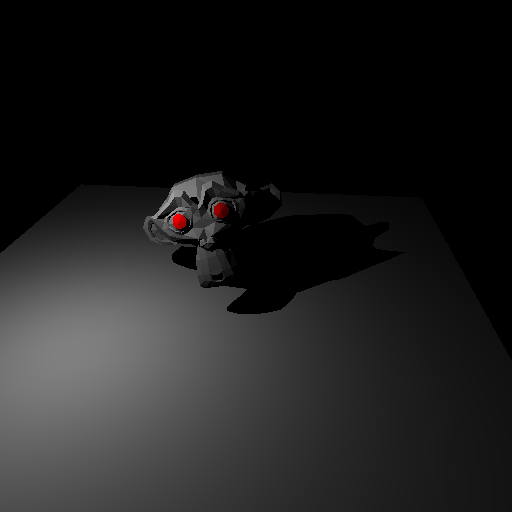
\includegraphics[width=.6\textwidth]{images/monkey.png}
  \caption{Monkey Szene}
\end{figure}
\begin{figure}
  \center
  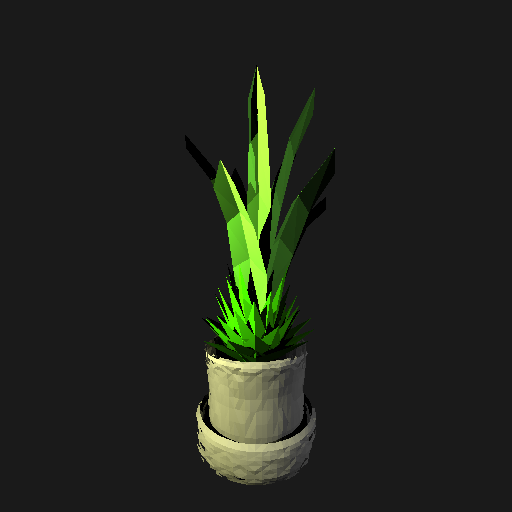
\includegraphics[width=.6\textwidth]{images/plant.png}
 \caption{Plant Szene}
\end{figure}
\begin{figure}
  \center
  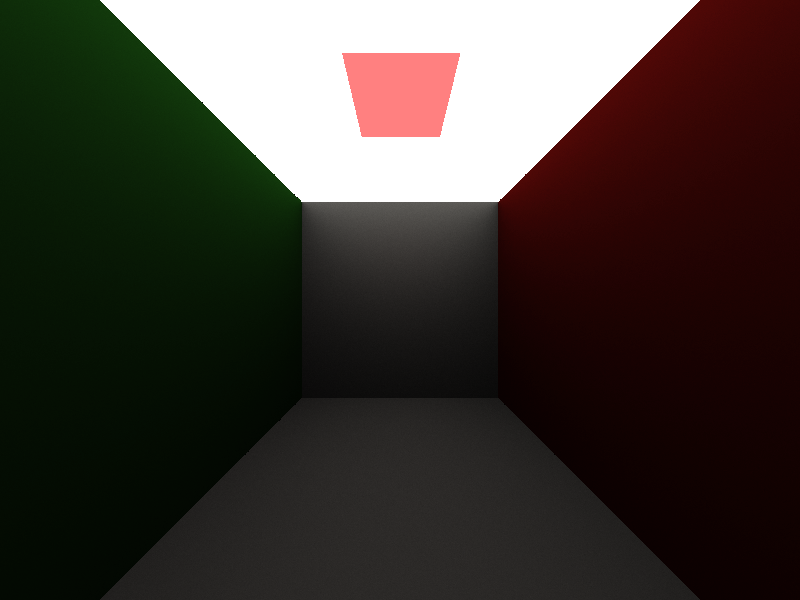
\includegraphics[width=.6\textwidth]{images/pt_cornell.png}
  \caption{PT/Cornell Szene}
\end{figure}
  
\subsection{Getestete Konfigurationen}
\subsection{Ergebnisse}
\begin{figure}
  \center
  \caption{Monkey Szene}
  \label{fig:runtime_monkey}
  \begin{tikzpicture}
  \begin{axis} [
    symbolic x coords={Baseline,Adaptive-Sampling,OpenMP,SSERay,BIH,KdTree,Kombiniert},
    table/header=false,
    enlargelimits=0.15,
    ymode=log,
    scaled y ticks = false,
    ylabel={Laufzeit (ms)},
    xtick=data,
    x tick label style={rotate=45,anchor=east},
  ]
      \addplot [box plot median] table {evaluation/monkey.dat};
      \addplot [box plot box] table {evaluation/monkey.dat};
      \addplot [box plot top whisker] table {evaluation/monkey.dat};
      \addplot [box plot bottom whisker] table {evaluation/monkey.dat};
  \end{axis}
  \end{tikzpicture}
\end{figure}

\begin{figure}
  \center
  \caption{Plant Szene}
  \label{fig:runtime_plant}
  \begin{tikzpicture}
  \begin{axis} [
    symbolic x coords={Baseline,Adaptive-Sampling,OpenMP,SSERay,BIH,KdTree,Kombiniert},
    table/header=false,
    enlargelimits=0.15,
    ymode=log,
    scaled y ticks = false,
    ylabel={Laufzeit (ms)},
    xtick=data,
    x tick label style={rotate=45,anchor=east},
  ]
      \addplot [box plot median] table {evaluation/plant.dat};
      \addplot [box plot box] table {evaluation/plant.dat};
      \addplot [box plot top whisker] table {evaluation/plant.dat};
      \addplot [box plot bottom whisker] table {evaluation/plant.dat};
  \end{axis}
  \end{tikzpicture}
\end{figure}

\begin{figure}
  \center
  \caption{PT/Cornell Szene}
  \label{fig:runtime_pt_cornell}
  \begin{tikzpicture}
  \begin{axis} [
    symbolic x coords={Baseline,Adaptive-Sampling,OpenMP,SSERay,Cuda,BIH,KdTree,Kombiniert},
    table/header=false,
    enlargelimits=0.15,
    ymode=log,
    scaled y ticks = false,
    ylabel={Laufzeit (ms)},
    xtick=data,
    x tick label style={rotate=45,anchor=east},
  ]
      \addplot [box plot median] table {evaluation/pt_cornell.dat};
      \addplot [box plot box] table {evaluation/pt_cornell.dat};
      \addplot [box plot top whisker] table {evaluation/pt_cornell.dat};
      \addplot [box plot bottom whisker] table {evaluation/pt_cornell.dat};
  \end{axis}
  \end{tikzpicture}
\end{figure}

\section{Fazit und Ausblick}


%Citation Page
\clearpage %Starts a new page to start new double page \cleardoublepage
%\bibliographystyle{apa}
\bibliographystyle{abbrvnat}

\bibliography{paper}
\clearpage
%Appendix
\begin{appendices}
\section{Some Appendix} %TODO write appendix sections here
The contents...
\end{appendices}





\end{document}
